\section{Imperfect Scaling Study}\label{sec:case-study}

This section focuses on a case study, which explores the frequency scaling 
capability of the system with two types of access patterns in applications.
An assumption often made, with respect to the power utilization 
is that on a given CPU, changing the frequency will change the CPU performance by the corresponding amount (generally called as scaling).
However, this is only true when considering the CPU execution. 
But, there are other architectural parameters whose performance do not scale along with CPU frequency.
One particular example would be memory. CPU caches hide much of this latency, but cache misses can be particularly damaging for the system energy efficiency,
as the time frame is too short for the operating system to handle the cache misses intelligently, or even be aware of them.
%except retrospectively, 
Yet, OSes take long enough time to make a decision that they measurably decrease the performance and/or efficiency.
 
To demonstrate this effect, we wrote a simple micro-benchmark, where a process takes large array (32MB), 
copies a random entry to another random entry in memory. 
We then operate the CPU at variety of frequencies using \texttt{CPUPOWER}~\cite{cpupower} utility and measured the execution time.  
This workload was then compared to another process that did the exact work of copying data from one point to another, but did so sequentially, avoiding most of the cache misses. 
As expected for both processes the time to execute decreases as CPU frequency increases.
We can then plot the \emph{efficiency}, computed  here as the time to execute the process
represented as the number of clock cycles per operation. For ease of comparison these were then normalized.
Figure~\ref{fig:case} shows the comparison of the random access workload with the sequential workload with increasing CPU frequency, normalized
to the base 1200Mhz frequency. 

\begin{figure}
  \begin{center}
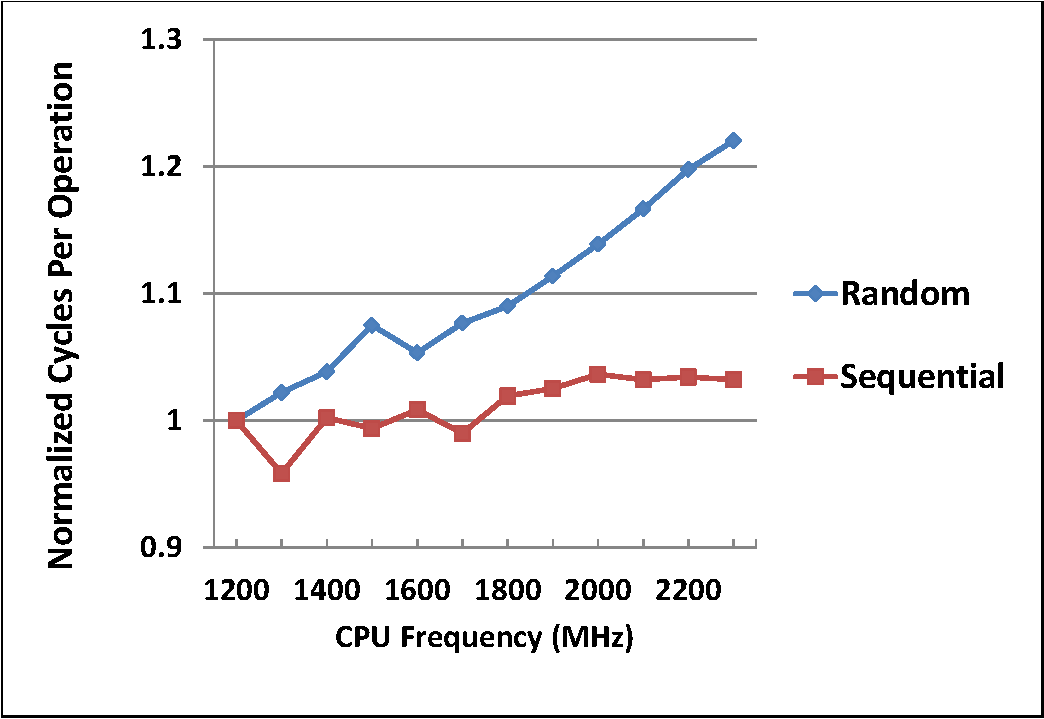
\includegraphics[width=\linewidth]{figs/case-crop.pdf}
  \end{center}
  \vspace{-0.1in}
  \caption{Frequency scaling effect for cache misses}
	\label{fig:case}
\end{figure}

\begin{figure*}[h]
  \begin{center}
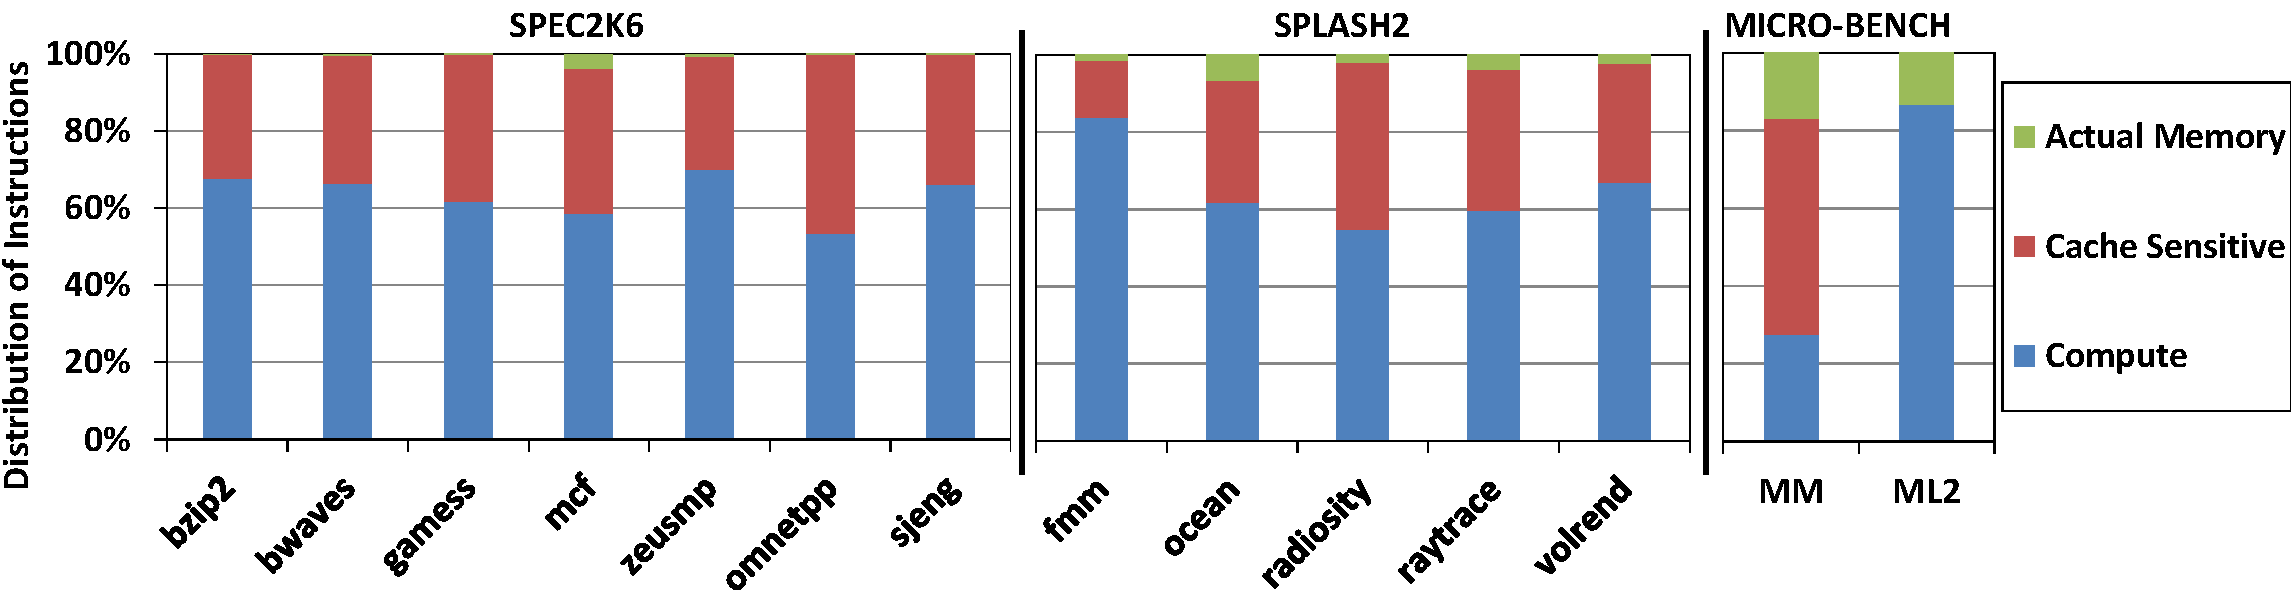
\includegraphics[width=\linewidth]{figs/app-cat-crop.pdf}
  \end{center}
  \vspace{-0.1in}
  \caption{Distribution of Instructions in Applications}
  \label{fig:app-cat}
\end{figure*}



Since both processes do the same amount of computation, the only factor that can affect the performance and efficiency is the memory access pattern. 
If the performance scaled perfectly with CPU frequency, we would expect a nearly flat line, with all cache hits
as we see in the case of sequential access workload in the figure. 
But with random accesses, we see instead that the cycles per operation increase as the frequency increases, 
clearly demonstrating a decrease in the efficiency. This is because of time spent in handling cache misses, and 
CPU is not doing any useful work to hide this latency.
It can be seen that at 2300Mhz, we are ~20\% less efficient than at 1200MHz.
There are two mitigating factors with respect to this issue. First is programming practices -- since cache misses are a well known performance issue, 
many applications are already written to avoid them as much as reasonable. Second is the hardware -- in particular modern processors have both hyperthreading and out of order execution, 
both of these features allowing the processor to potentially work on other instructions while the cache misses
are being served. 

Operating systems however, in this scenario does not take efficient decisions, to actually save energy 
by overriding the default policies. Instead, it still relies on its power
governors to run at higher CPU frequency and thus waste energy. This could be a simple
example, but nonetheless, as we will demonstrate in further sections  with some real workloads, 
the inevitable constraint is memory bandwidth and/or latency, and in these cases a decrease in CPU frequency may very well lead to efficiency gains.



